%In this section you will discuss the Technical Development related to your project.
%In one or more chapters you must describe fully the design and development strategies you have adopted and the results achieved.  You may refer to appropriate User and System documentation presented as appendices to avoid repeating extensive detail, so you can focus here instead on a discussion of your reasons for adopting the techniques and strategies you have followed.
%Again, it is difficult to give prescriptive guidance on the subsection structure you might adopt, as this will depend on the nature and content of your project.  However, you will probably want at least to consider sections addressing issues of System Design; Implementation; Testing.  If there is a lot to cover in any of these areas, it may warrant presentation as a full chapter rather than a section.
\chapter{Technical Development}



%System design:
%This can include UML diagrams such as class diagrams, use case diagrams, activity diagrams, etc.
%If you find that these are taking up a lot of space/words, then you should prioritise and relegate where appropriate to the appendices. 
%This should not just be a list of unexplained diagrams, but should rather include discussions of the most interesting parts of your design, tying them to your background and objectives.
\section{System design}



%UI design:%
%If your software includes user interaction then you could also include a discussion (supported by diagrams) of decisions that you have made regarding the user interface.%
\section{UI design}



%Experimental design:
%If you project includes any experiments, including but not limited to user testing, then you can discuss their design here. Note that again this does not exist in a vacuum and should be tied to your research.
\section{Experiential design}

\subsubsection{Packet Loss and its effect on download speeds}

% Better graph needed
\begin{center}
	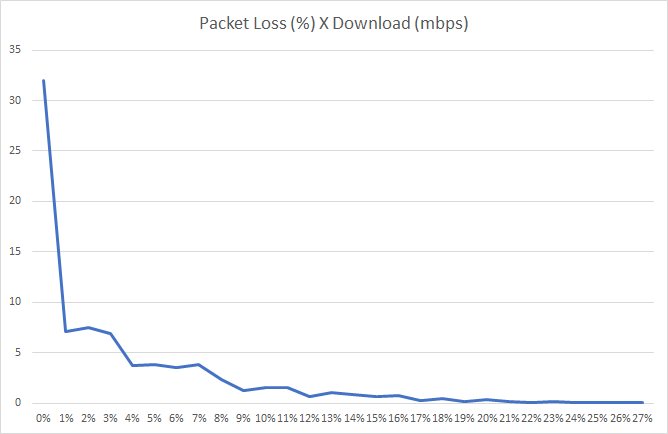
\includegraphics[scale=0.6]{PL_Download}
	\begin{figure}[h]
	 	\caption{Graph displaying effect of packet loss on download speeds}
	\end{figure}		
\end{center}

The graph above shows the download speed measured in Mbps against the increasing rate of packet loss, as you can see the download rate only reaches 28\%, this is due to the connection test failing at anything above. The tests were performed by querying the SpeedTest.net \comments{CITE} API. 

My initial hypothesis for the sharp decreases in packet loss from 0\% to 1\% is it's due to the congestion control mechanisms built into TCP. TCP as mentioned in the background section allows for multiple devices to co-exist on a network and dynamically balance network resources through congestion control algorithms, but packet loss in this aspect is assumed as a sign of congestion to the algorithm adapts and reduces its transfer rate each time a packet is lost, this means the transfer rate drastically reduces until it reaches a platform.

%The test for this will check the transfer rate over a period of time where it will drop a packet every 10 seconds and hopefully will see a dip in transfer rate when each packet is dropped

\comments{Decide on an experiment to prove this}
\comments{Also talk about why the transfer fails when the packet loss reaches 28\%}

\subsubsection{Latency and retransmission}

\comments{Graph here showing linear retransmission against increasing latency value}
The expected result from this graph was a large peak at the time out period where all the packets send would flag up as retransmissions. This graph is flat due to the dynamic way that TCP works out its RTO (Retransmission Timeout) value that includes the Round trip time (i.e) and this test that created the graph above has the latency affecting the entire time to the dynamic value of the RTO was using the latency value to calculate it and therefore meant that changing the value of latency had no effect 

% ## Reading
% https://tools.ietf.org/html/rfc6298
% https://sgros.blogspot.co.uk/2012/02/calculating-tcp-rto.html
% https://blog.catchpoint.com/2014/04/29/understanding-rtt-impact-on-tcp-retransmissions/

% Maybe a test where the handshake has not latency on it?
% Then the latency is increased to a cetain value 

\comments{Changing value of latency won't ever stop a TCP connection??}


%Test design and system testing:
%Testing is an extremely important part of any software project and should not be a tacked on afterthought. You can include here a discussion of the design of any tests that you intend to carry out on your project. It would not be appropriate to include an exhaustive list of all the individual tests that you wish to conduct (consider the appendices for this) but examples would be useful to illustrate your discussion.
%You should review how you have approached the testing and quality assurance of your delivered product, including relevant choice of incremental and/or integration testing, test scenarios, sample datasets, etc. as appropriate,  Exhaustive reproduction of extensive test records is not required, but sample evidence should be used to support your discussion.
\section{Test design and system testing}



%System Implementation:$
%You should review how you have implemented your project system, discussing any areas of the implementation which might for example involve code or processes which are not immediately obvious in structure or operation, where you have had to innovate or develop particular approaches.  Again, you should refer to relevant diagrams of code or object structures which should be included in documentation as appended.
\section{System Implementation}

